%!TEX root = Report.tex
\chapter{Introduction}\label{sec:introduction}
Schlieren photography is a powerful technique to visualize density and temperature variations in flows. It was invented 1864 by August Toepler to examine supersonic motion. Schlieren technology is based on the principle of light being bent by refractive index variations due to the different propagation speed of light. $n=\frac{c_0}{c}$ 

\section{Optical Density Measurements}
The classical Schlieren technology consists of a point source of illumination, several lenses, a test section and a camera as depicted in Figure \ref{pic:Setup_optical}. \\
\begin{figure}[H]
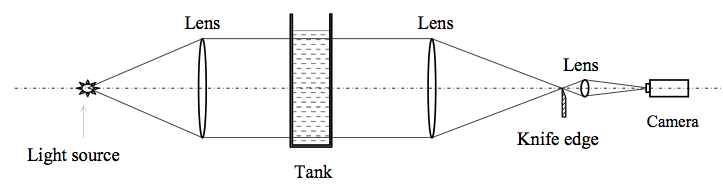
\includegraphics[width=1\textwidth]{pics/Setup_optical.png}
\caption{Working Principle Optical Schlieren - \emph{Source:} \cite{thomas2009synthetic}}
\label{pic:Setup_optical}
\end{figure}

In the test section the collimated light beam is distorted by density gradients in the fluid. Distortions create spatial variations in light intensity and the "knife" stops the rays deviated from parallelism. Though all Schlieren technologies have the huge advantage of being non-invasive there are several difficulties to this technique. First of all the experimental setup of positioning the lenses is complicated, sensitive to disturbances and fairly expensive. Furthermore the emitted light from a single-point source is limited as well as the size of lenses. Finally direct quantitative analysis remains difficult due to the fact that all information is encoded in brightness and no absolute reference is available.

\section{Schlieren measurements, Examples Of Use}

Background Oriented Schlieren (BOS), first introduced in the late 1990's, is a much simpler technique of the larger field of Synthetic Schlieren. Just as the optical Schlieren method it is commonly used for two-dimensional flow visualizations of temperature and density changes in several fields, such as fluid mechanics, ballistics, heat exchange through convection, as well as observing the propagation and mixing behavior of gases. Latest developments of this technique even allow precise quantitative visualization of fluid flows, coupling the refractive index with flow properties.

\section{Working Principle Of Synthetic Schlieren Method}

As mentioned earlier the setup for the Synthetic Schlieren technique is much simpler than one of the Optical Schlieren method. Beams from the diffuse light source pass through a mask and are captured by a digital camera as illustrated in Figure \ref{pic:Setup_synthetic}. A reference picture (without test section) is compared with one containing the test section.
\begin{figure}[H]
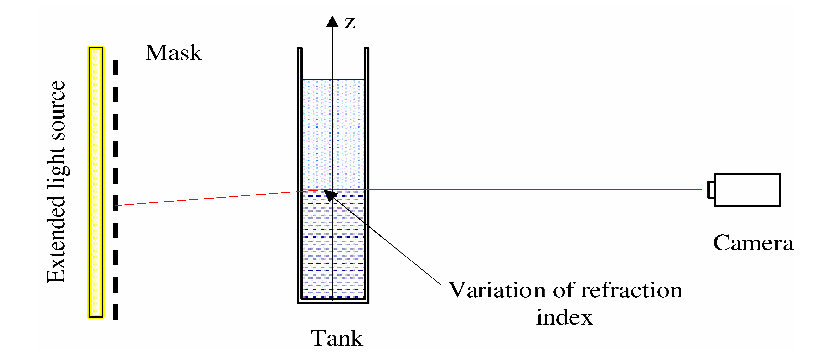
\includegraphics[width=1\textwidth]{pics/Setup_synthetic.png}
\caption{Working Principle Synthetic Schlieren - \emph{Source:} \cite{thomas2009synthetic}}
\label{pic:Setup_synthetic}
\end{figure}
The improvements are obvious. No expensive mirrors, lenses and no single-point source of light is needed. The technique of Background Oriented Schlieren (BOS) is even simpler. Instead of an extended light source and a mask only a random background pattern is needed.\\
To derive from optical distortions to temperature or density variations, a relation between refractive index and fluid properties is needed. The "Gladstone-Dale" relationship 
\begin{equation}
n-1 = K \cdot \rho = K \cdot \frac{p}{RT}
\end{equation}
provides such link for gases. The empirical relationship for paraffin oil used in the experiment is shown below.
\begin{equation}
n(T)= 1.48-0.00036 \cdot T(^\circ C)
\label{eq:nparafin}
\end{equation}

